\section{Análisis y discusión de los resultados obtenidos}\label{sec:cs-resultados-de-la-encuesta}

La encuesta fue diseñada para tener 14 preguntas orientadas a detectar y/o descartar la necesidad de tener la carrera de Ciencia de la Computación en nuestro pa­s.

El análisis presentado a continuación está basado en los resultados de las respuestas válidas obtenidas a partir de las encuestas realizadas a los diferentes empresarios de nuestro medio. Las preguntas que no fueron respondidas (en blanco) no están consideradas en los gráficos.

La pregunta 1, tiene un carácter netamente informativo y podemos ver que una gran mayor­a de las empresas encuestadas efectivamente necesitan profesionales formados a nivel universitario en el área de computación.

\newcommand{\mywidth}{10cm}

\begin{figure}[!h]
	\centering
	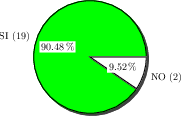
\includegraphics[]{\OutputFigsDir/Pregunta1}
	\label{fig:Preg1}
	\caption{?`Usted necesita en su empresa profesionales en el área de computación formados a nivel universitario?}
\end{figure}


En la pregunta 2, es necesario resaltar que un porcentaje muy alto de empresarios, más de la mitad, no conocen bien la diferencia entre los perfiles profesionales en el área de computación que existen internacional y localmente. La preocupación en este caso se debe que el porcentaje de los que no conocen deber­a ser inexistente. Este mismo resultado nos plantea una nueva necesidad de difundir correctamente los perfiles hacia el mundo empresarial.


\begin{figure}[!h]
	\centering
	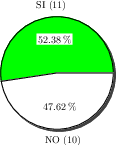
\includegraphics[]{\OutputFigsDir/Pregunta2}
	\label{fig:Preg2}
	\caption{?`Podr­a usted diferenciar los perfiles profesionales de Ingenier­a de Sistemas, Ciencia de la Computación, Ingenier­a del Software, Tecnolog­as de Información, Sistemas de Información e Ingenier­a Informática?}
\end{figure}

En la pregunta 3, sobre el nivel de auto percepción de la competitividad de sus empresas, nuestros encuestados indicaron que no se consideran competitivos en su mayor­a. Este resultado nuevamente nos abre la pregunta: ?`Es posible afirmar que estamos formando profesionales competitivos si los propios empresarios no lo consideran as­?

\begin{figure}[!h]
	\centering
	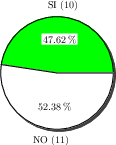
\includegraphics[]{\OutputFigsDir/Pregunta3}
	\label{fig:Preg3}
	\caption{En el contexto del libre comercio y globalización en que vivimos, ?`Usted considera que su empresa es tecnológicamente competitiva?}
\end{figure}

En la pregunta 4, sobre su conocimiento de la existencia de estándares internacionales en el área de computación, los empresarios manifestaron, en su gran mayor­a, que conocen de la existencia de los mismos. Sin embargo también es lógico pensar que, por no ser espec­ficamente del área, ese conocimiento no necesariamente implica una definición clara por parte de los mismos. Esto puede claramente ser contrastado con el resultado obtenido en la pregunta 2.


\begin{figure}[!h]
	\centering
	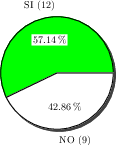
\includegraphics[]{\OutputFigsDir/Pregunta4}
	\label{fig:Preg4}
	\caption{?`Sabe usted que existen los estándares internacionales bajo los cuales se forman profesionales del área de computación (Ingenier­a de Computadores, Ciencia de la Computación, Ingenier­a del Software, Tecnolog­as de Información, Sistemas de Información)?}
\end{figure}

La pregunta 5, está relacionada al saber quién creen nuestros empresarios que son los responsables por la correcta difusión de los perfiles de la carrera. Esta pregunta fue diseñada para que el encuestado escoja más de una opción, si fuera necesario. El punto importante es que el total de nuestros encuestados señalaron a la universidad como primer responsable de dicha difusión y a los colegios profesionales en segundo lugar con menos de la mitad de los casos. Esta pregunta también nos hace percibir que hace falta una mayor coordinación entre estas dos instituciones, universidad y colegios profesionales, tomando siempre como base los estándares internacionales que rigen a las carreras.

\begin{figure}[!h]
	\centering
	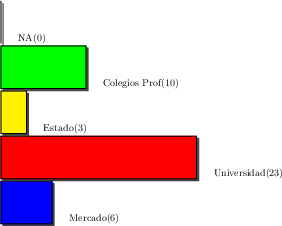
\includegraphics[width=5cm,height=5cm]{\OutputFigsDir/Pregunta5}
	\label{fig:Preg5}
	\caption{?`De quién cree usted que es la responsabilidad de la correcta difusión de los perfiles de formación profesional existentes?}
\end{figure}

La pregunta 6, tiene por objetivo demostrar que el empresario no sólo necesita profesionales que apliquen tecnolog­a para la solución de problemas. La percepción que tienen los empresarios es que la innovación permanente es muy importante en más de un 90\%. En ningún caso se obtuvo que el hecho de ser innovador fuese nada importante. Esta es una caracter­stica que es percibida como muy importante y necesaria en nuestros egresados. En este gráfico también debemos recordar que la innovación permanente es una caracter­stica muy presente en el profesional de Ciencia de la Computación.

\begin{figure}[!h]
	\centering
	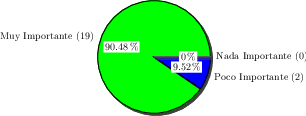
\includegraphics[]{\OutputFigsDir/Pregunta6}
	\label{fig:Preg6}
	\caption{?`Qué tan importante es la innovación permanente en su empresa, para el logro de sus objetivos?}
\end{figure}

Antes de esta encuesta era muy común escuchar que los profesionales del área de computación deben siempre estar orientados a la aplicación de tecnolog­as. Sin embargo, la pregunta 7, nos demuestra de forma contundente que la formación de investigador es necesaria para la industria de software. Esto tiene que ver con el hecho de innovar a través de la búsqueda de nuevas soluciones basadas en investigaciones. Este resultado es particularmente importante si deseamos que nuestro pa­s deje gradualmente la dependencia tecnológica que presenta para pasar a ser un pa­s generador de nuestra propia tecnolog­a.

\begin{figure}[!h]
	\centering
	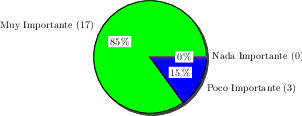
\includegraphics[]{\OutputFigsDir/Pregunta7}
	\label{fig:Preg7}
	\caption{?`Qué tan importante es que sus profesionales sean también investigadores que planteen nuevas soluciones?}
\end{figure}

La pregunta 8, demuestra que los empresarios sienten que habr­a una clara ventaja competitiva si sus profesionales fuesen creadores e innovadores de tecnolog­a computacional. Aqu­ vemos claramente una necesidad no cubierta, que podr­a ser cubierta por el perfil propuesto en este documento ya que el profesional en Ciencia de la Computación esta principalmente orientado a estos puntos: creación e innovación de tecnolog­a computacional.

\begin{figure}[!h]
	\centering
	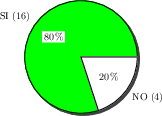
\includegraphics[]{\OutputFigsDir/Pregunta8}
	\label{fig:Preg8}
	\caption{?`Considera usted que obtendr­a ventaja competitiva en el mercado, si su empresa contara con profesionales que fuesen creadores e innovadores de tecnolog­a computacional?}
\end{figure}

La necesidad de la detección patrones no obvios, planteada en la pregunta 9,  es un tipo de preparación que va más allá de saber manipular una base de datos. Este tipo de preparación tiene que ver con el tema de \textit{Data Mining} y \textit{Web Mining} que actualmente no se hace con mucha profundidad en nuestro pa­s.

Una de las mayores razones por las cuáles la computación ha pasado a ser tan importante en nuestras vidas es la aparición de la Internet o productos tan populares como los buscadores Google y Yahoo!. Un gran responsable de este cambio en nuestras vidas es sin duda la propuesta de productos Microsoft que actualmente son muy utilizados en todo el planeta. 

Sin embargo, una cosa es saber usar esos productos y otra cosa es saber hacerlos. El éxito de empresas como Microsoft es sin duda que ellos se orientaron a crear esa tecnolog­a a nivel de micro computadores. El perfil profesional que domina este mercado de creadores, es el de Ciencia de la Computación e Ingenier­a de Software. En este último caso es posible ir más a fondo en el tema y observar que empresas como Google consideran que para cubrir el cargo de Ingeniero de Software la formación básica debe ser en Ciencia de la Computación. Esto mismo sucede en una gran mayor­a de empresas de este tipo.

\begin{figure}[!h]
	\centering
	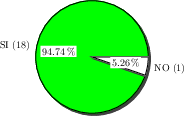
\includegraphics[]{\OutputFigsDir/Pregunta9}
	\label{fig:Preg9}
	\caption{?`Le gustar­a contar con profesionales que estén capacitados para detectar patrones de comportamiento no obvios en sus clientes que le permitan tomar decisiones al nivel estratégico de su empresa?}
\end{figure}

Los resultados obtenidos de la pregunta 10, nos confirman que el empresariado peruano también tiene ese aspecto en claro. Si consideramos el procentaje de empresarios que relacionan este tipo de productos con Ciencia de la Computación e Ingenier­a de Software tenemos un porcentaje que supera un 80\%.

Esta misma pregunta 10, también nos ha permitido observar un resultado inesperado y es que el empresariado tiene claro que este tipo de productos NO son creados por Ingenieros de Sistemas y tampoco por Ingenieros Informáticos que en ambos casos no tuvieron ningún voto a favor.

\begin{figure}[!h]
	\centering
	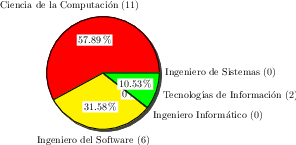
\includegraphics[]{\OutputFigsDir/Pregunta10}
	\label{fig:Preg10}
	\caption{?`Qué tipo de profesional cree usted que es aquel que ha creado Internet, el buscador Google, el sistema operativo (Windows, Linux), Microsoft Office (Word, Excel, PowerPoint) y las bases de datos (Oracle, SQL Server, MySql)?}
\end{figure}

La pregunta 11, refleja otro resultado interesante. Según la opinión de nuestros empresarios el tipo de profesionales antes mencionados son muy relevantes y relevantes en más de un 90\%. Nuestros empresarios claramente relacionan, estos profesionales, con un fuerte eje de desarrollo de la industria de software. La ausencia de estos profesionales también podr­a ser la causa del lento despegue de esta industria en nuestro pa­s y vale la pena reflexionar al respecto.

\begin{figure}[!h]
	\centering
	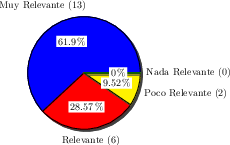
\includegraphics[]{\OutputFigsDir/Pregunta11}
	\label{fig:Preg11}
	\caption{?`Qué tipo de profesional cree usted que es aquel que ha creado Internet, el buscador Google, el sistema operativo (Windows, Linux), Microsoft Office (Word, Excel, PowerPoint) y las bases de datos (Oracle, SQL Server, MySql)?}
\end{figure}

La pregunta 12, tiene por objetivo detectar si estos mismos empresarios se sentir­an atra­dos para invertir en profesionales que estuvieran preparados para generar el software antes mencionado. La respuesta ha sido positiva en más de 75\% y nos permite confirmar que en nuestro medio hay dinero disponible para impulsar esta industria y que lo que falta es el profesional preparado para ese perfil profesional.

\begin{figure}[!h]
	\centering
	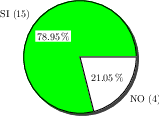
\includegraphics[]{\OutputFigsDir/Pregunta12}
	\label{fig:Preg12}
	\caption{?`Si tuviéramos este tipo de profesionales, usted considerar­a interesante invertir en este rubro?}
\end{figure}

Estos mismos empresarios fueron cuestionados sobre si conocen o no alguna empresa en Perú que este preparada para producir la tecnolog­a computacional que actualmente compramos del exterior. En esta pregunta se esperaba que por lo menos hubiese indicios de que aqu­ se pueda crear esa tecnolog­a. Sin embargo, una gran mayor­a de los encuestados manifestaron que no conocen empresas que esten en capacidad de poder generar software con calidad internacional. Todo esto se ve claramente reflejado en los resultados de la pregunta 13.

\begin{figure}[!h]
	\centering
	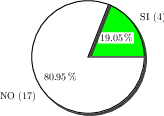
\includegraphics[]{\OutputFigsDir/Pregunta13}
	\label{fig:Preg13}
	\caption{?`Conoce alguna empresa en Perú que sea capaz de crear la tecnolog­a computacional que su empresa compra actualmente con calidad internacional?}
\end{figure}

En la última pregunta se cuestionó sobre la importancia de tener este tipo de empresas para el desarrollo nacional. A pesar de no generar este tipo de software en Perú en este instante, observamos que la totalidad de empresarios peruanos consideran que es muy importante o importante contar con este tipo de empresas.

\begin{figure}[!h]
	\centering
	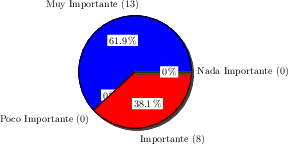
\includegraphics[]{\OutputFigsDir/Pregunta14}
	\label{fig:Preg14}
	\caption{?`Qué tan importante considera usted que existan ese tipo de empresas para el desarrollo nacional?}
\end{figure}


